% LaTeX file for Chapter 02









\chapter{Methodology} 

\section{Definitions}

The \textbf{Target Population} is a specific group within the broader population, defined by attributes relevant to the research question. This group is selected based on criteria that match the study's goals, helping researchers focus on the most pertinent segments of the population \citep{willie2024population}. Defining the target population allows researchers to refine their objectives and sampling methods to align with the study's aims.


The \textbf{Eligibility} criteria are the specific requirements that individuals must meet to participate in a study. Eligible patients will be selected from the target population. It is important to note that eligibility criteria also include exclusion factors, conditions or circumstances that disqualify potential participants \citep{food2018evaluating}. Inclusion criteria specify the conditions that allow individuals to participate in the trial, particularly focusing on the medical condition of interest. Any other factors that limit eligibility are classified as exclusion criteria \citep{van2007eligibility}.


In clinical trials, \textbf{Enrollment} refers to the formal process of registering participants into a study after they have met all eligibility criteria and provided informed consent. This process includes verifying that each participant satisfies the inclusion and exclusion criteria outlined in the study protocol \citep{NIH2021}. It is important to distinguish between recruitment and enrollment. Recruitment involves identifying and inviting potential participants to join the study, whereas enrollment occurs after these individuals have been screened, consented, and officially registered into the trial \citep{frank2004current}. 

Once enrolled, participants are assigned to specific treatment groups or interventions as defined by the study design. The most common practice been \textbf{Randomization}. In clinical research, randomization is the process of assigning participants to different treatment groups using chance methods, such as random number generators or coin flips \citep{lim2019randomization}. Randomized controlled trials (RCTs) are considered the most effective method for preventing bias in the evaluation of new interventions, drugs, or devices. \citep{van2007eligibility}.


In clinical research, \textbf{Statistical Analysis} involves applying statistical methods to collect, summarize, interpret, and present data derived from clinical studies. This process is essential for evaluating the safety, efficacy, and overall outcomes of medical interventions, ensuring that conclusions drawn are both reliable and valid \citep{panos2023statistical}. Not all participants who are randomized may be included in the final statistical analysis due to protocol deviations of patients not adhering to the protocol \citep{rehman2020exclusion}, missing data \citep{shih2002problems} or loss-to-follow-up, some participants may become unreachable or withdraw consent during the study, resulting in missing outcome data \citep{nuesch2009effects}.

\begin{figure}[h]
  \centering
  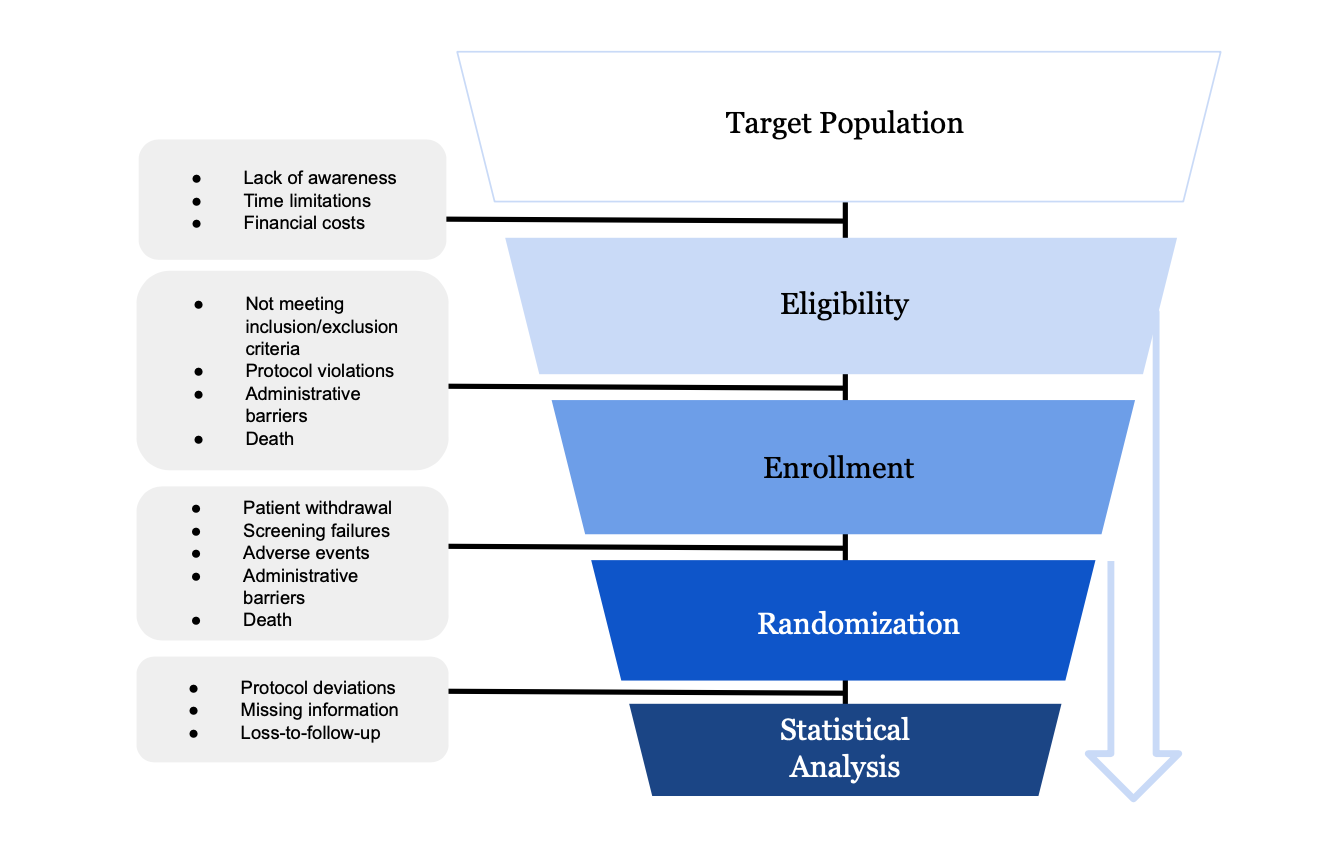
\includegraphics[width=0.7\textwidth]{fig_2_1.png}
  \caption{Patient Attrition at Each Stage of a Clinical Study. References: \cite{piantadosi2022principles, whelan2018high, bogin2022lasagna}}
  \label{fig:2_1}
\end{figure}

The number of patients decreases at each stage of a clinical study, from defining the target population to final statistical analysis, see Figure \ref{fig:2_1}. Eligibility criteria narrow down participants, and enrollment further reduces numbers as only those meeting strict criteria are registered. Randomization assigns individuals to treatment groups, but some may later be excluded due to protocol deviations, missing data, or loss to follow-up. 


\section{Uncertainty and models for counts}

Let us define \textbf{Aleatory Uncertainty} as that which can be characterised by randomness. It is inherent, irreducible and unpredictable in nature. Whereas \textbf{Epistemic Uncertainty} arises primarily from limited or imperfect knowledge and can be reducible by obtaininng more or better information. 

Let us denote

\begin{itemize}
\item $T=time$
\item $C=counts$
\item $\lambda=\frac{C}{T}$
\end{itemize}

\begin{table}[h!]
\centering
\resizebox{\textwidth}{!}{
\begin{tabular}{cccccc}
 \textbf{Methods} & \textbf{Counts} & \textbf{Expectation} & \textbf{Variance} & \textbf{Aleatory} & \textbf{Epistemic} \\
\hline
\hline
Expectation & $C = \lambda  T$ & $\lambda  T$ & 0 & No & No \\
Poisson & $C \sim \text{Po} (\lambda  T)$ & $\lambda  T$ & $\lambda  T$ & Yes & No \\
Negative Binomial & $C \sim \text{Po} (\Lambda  T)$; $\Lambda \sim G(\alpha,\beta)$ & $\frac{\alpha}{\beta}$ & $\frac{\alpha(\beta+1)}{\beta^2}$ & Yes & Yes \\
\end{tabular}
}
\caption{Aleatory and epistemic uncertainty shown by different models for counts.}
\label{tab:count_modeling}
\end{table}

\begin{figure}
\begin{knitrout}
\definecolor{shadecolor}{rgb}{0.98, 0.98, 0.98}\color{fgcolor}

{\centering 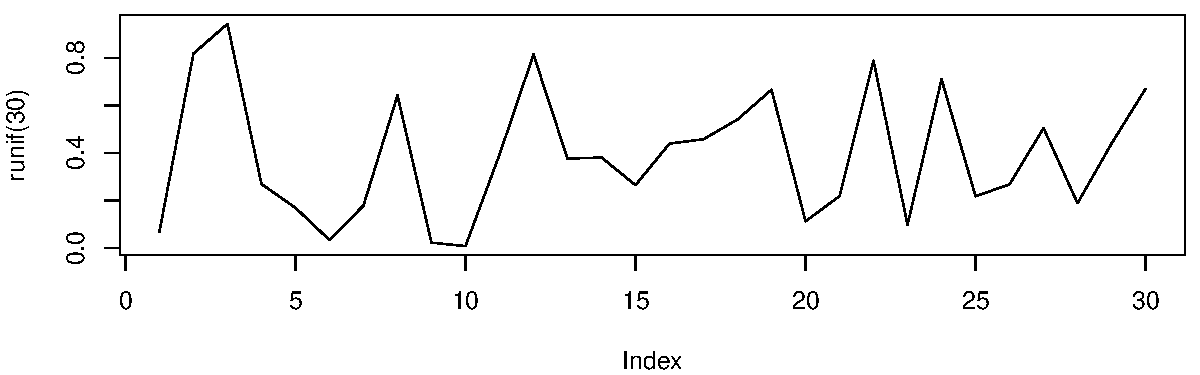
\includegraphics[width=\textwidth-3cm]{figure/ch02_figunnamed-chunk-3-1} 

}


\end{knitrout}
  \caption{Poisson-distributed counts over time and uncertainty range. The black line represents the point estimate expectation ($\lambda = 15$), while the grey dashed lines indicate Poisson's 95\% aleatory uncertainty. The histogram illustrates the distribution of observed counts at time $T = 40$. Ref.: \cite{spiegelhalter2011visualizing}.}
  \label{fig:2_2}
\end{figure}


\begin{figure}
\begin{knitrout}
\definecolor{shadecolor}{rgb}{0.98, 0.98, 0.98}\color{fgcolor}

{\centering 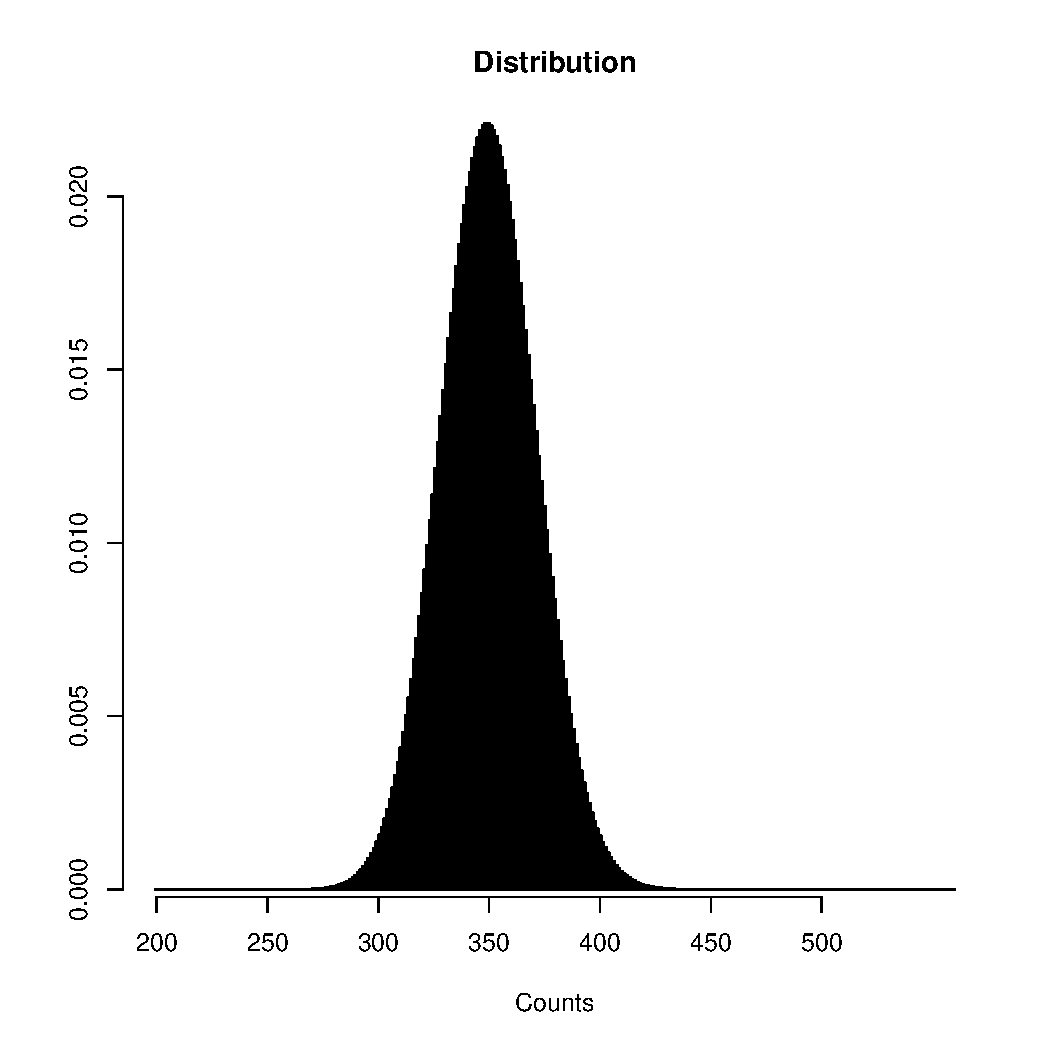
\includegraphics[width=\textwidth-3cm]{figure/ch02_figunnamed-chunk-4-1} 

}


\end{knitrout}
  \caption{Predicted uncertainty bands for poisson process over time. The black line represents the mean trend $\lambda = 15$, while the green shaded regions indicate aleatory uncertainty: the dark green band spans the interquantile range (25th - 75th percentiles), the lighter green band cover the 10th - 90th percentile range and the light green the 2.5th - 97.5th percentile range. Ref.: \cite{spiegelhalter2011visualizing}.}
  \label{fig:2_3}
\end{figure}



\section{Derivation of Negative Binomial from Poisson-Gamma model}

Let $Y|\lambda \sim Po(\lambda)$ and $\lambda \sim G(\alpha,\beta)$
\begin{align*}
p(y)&=\int^\infty_0 p(y|\lambda) p(\lambda) d\lambda\\
&=\int^\infty_0 \frac{\lambda^y\exp(-\lambda)}{y!}\Bigg[\lambda^{\alpha-1}\exp(-\beta\lambda)\frac{\beta^\alpha}{\Gamma(\alpha)}\Bigg]d\lambda\\
&=\frac{\beta^\alpha}{y!\Gamma(\alpha)}\int^\infty_0 \lambda^{\alpha+y-1}\exp(-\lambda)\exp(-\lambda\beta)d\lambda\\
&=\frac{\Gamma(\alpha+y)}{y!\Gamma(\alpha)}\int^\infty_0 \beta^\alpha \exp(-\lambda\beta)d\lambda\\
&=\frac{\Gamma(\alpha+y)}{y!\Gamma(\alpha)}\Bigg(1-\frac{\beta}{\beta+1}\Bigg)^{\alpha}\Bigg(\frac{\beta}{\beta+1}\Bigg)^y \sim NBin \Bigg(\alpha, \frac{\beta}{\beta+1}\Bigg)
\end{align*}

To calculate the mean and variance:

\begin{align*}
Mean &= \frac{\alpha\bigg(1-\frac{\beta}{\beta+1}\bigg)}{\frac{\beta}{\beta+1}}\\
&= \frac{\alpha\bigg (\frac{1}{\beta+1}\bigg)}{\frac{\beta}{\beta+1}}\\
&= \frac{\alpha(\beta+1)}{\beta(\beta+1)}\\
&= \frac{\alpha}{\beta}
\end{align*}

\begin{align*}
Variance &= \frac{\alpha\bigg(1-\frac{\beta}{\beta+1}\bigg)}{\bigg(\frac{\beta}{\beta+1}\bigg)^2}\\
&= \frac{\alpha\bigg (\frac{1}{\beta+1}\bigg)}{\bigg(\frac{\beta}{\beta+1}\bigg)^2}\\
&= \frac{\alpha(\beta+1)^2}{\beta^2(\beta+1)}\\
&= \frac{\alpha(\beta+1)}{\beta^2}
\end{align*}




